\documentclass[8pt]{extarticle}
\usepackage{multicol,caption}
\usepackage[utf8]{inputenc}
\usepackage[english]{babel}
\usepackage[a4paper, landscape, margin=1cm, footskip=0.7cm]{geometry}
\usepackage{graphicx}
\usepackage{lipsum}
\usepackage{amsmath}
\usepackage{dsfont}
\usepackage{gensymb}
\usepackage{mathrsfs}
\usepackage{framed}
\usepackage{enumerate}
\usepackage{array}
\usepackage{datetime}
\usepackage{calligra}
\usepackage[dvipsnames]{xcolor}
\usepackage[titles]{tocloft}
\usepackage[sfdefault]{roboto}
\usepackage{enumitem}
\usepackage[compact]{titlesec}
\usepackage{textcomp}


\setenumerate{itemsep=0pt,topsep=0pt}
\setitemize{itemsep=0pt, topsep=0pt}

\setlength{\parskip}{0cm}
\setlength{\parindent}{0em}
%\setlength{\headsep}{0pt}
\setlength{\topskip}{0pt}
%\setlength{\topmargin}{0pt}
\setlength{\topsep}{0pt}
\setlength{\partopsep}{0pt}

%% TOC
\graphicspath{{figures/}}

\makeatletter
\newenvironment{Table}
   {\par\bigskip\noindent\minipage{\columnwidth}\centering}
   {\endminipage\par\bigskip}
\makeatother

\setlist{nolistsep}


\newenvironment{Figure}
  {\par\medskip\noindent\minipage{\linewidth}}
  {\endminipage\par\medskip}

\newenvironment{conditions}
{\par\vspace{\abovedisplayskip}\noindent\begin{tabular}{>{$}l<{$} @{${}={}$} l}}
{\end{tabular}\par\vspace{\belowdisplayskip}}

\setlength{\columnseprule}{0.2pt}
\setlength{\columnsep}{10pt}
\renewcommand{\columnseprulecolor}{\color{lightgray}}

% TOC
\setlength{\cftbeforesecskip}{-.2ex}



\begin{document}

\begin{multicols}{3}
\noindent
\large Virtual Reality
\normalsize \\
\today, \currenttime

\section{Tipologie di occhiali}
\subsection{Occhiali 3D attivi di tipo shutter}
\paragraph{Nomi alternativi} Active Shutter 3D System, Alternate Frame Sequencing, Alternate Image,
AI, Alternating Field, FIeld Sequential, Eclipse Method.

\paragraph{Descrizione} Tecnica utilizzata per mostrare immagini stereoscopiche in 3D.
Funziona mostrando immagini differenti per ogni occhio, bloccando sequenzialmente un'occhio alla volta
e permettendo all'altro di visualizzare l'immagine. L'operazione è talmente veloce che le interruzioni
non interferiscono con la fusione percepita delle due immagini 3D.

Gli occhiali ad otturatore attivo di nuova generazione generalmente usano degli otturatori a cristalli
liquidi (anche chiamati "LC Shutter Glasses"). Ogni lente dell'occhiale contiene uno strato di
cristallo liquido che ha la proprietà di diventare opaco quando viene applicata della tensione,
altrimenti resta trasparente. In questo modo, tramite un segnale di clock, gli occhialini
cambiano di stato (visione occhio destro, visione occhio sinistro). Questo segnale di clock può
essere mandato attraverso un cavo, oppure senza fili con infrarossi o tramite
trasmettitori a radio frequenza (Bluetooth, DLP link).

\paragraph{Vantaggi} 
\begin{itemize}
    \item A differenza degli occhialini a filtri rosso/ciano (anaglifi), gli occhialini
    attivi di tipo shutter non influenzano il colore, permettendo così di visualizzare le
    immagine a pieno spettro cromatico. Tramite l'utilizzo di ColorCode, i sistemi ad anaglifi
    arrivano a risultati simili fornendo una risoluzione cromatica completa.

    \item A differenza dei sistemi 3D polarizzati, dove generalmente la risoluzione
    orizzontale è dimezzata, gli occhialini attivi di tipo shutter possono mantenere
    una risoluzione piena per entrambe le immagini. 
\end{itemize}

\paragraph{Svantaggi}
\begin{itemize}
    \item È possibile notare del flickering, tranne quando si utilizza un refresh rate molto alto,
    in quanto ogni occhio sta effettivamente ricevendo solo la metà del refresh rate effettivo dello
    schermo. Ad ogni modo, gli occhialini LC moderni funzionano generalmente a refresh rate più alti
    ed eliminano quindi il problema per la maggior parte delle persone.
    \item Fino a poco tempo fa questo metodo funzionava solo con monitor di tipo CRT; alcuni
    flat-panel moderni supportano ora un refresh rate abbastanza elevato per funzionare con 
    alcuni sistemi LC. Molti proiettori, specie quelli basati su DLP, includono la
    funzionalità di 3D.
    \item Gli occhiali LC otturano la luce per la metà del tempo, inoltre fanno passare leggermente
    meno luce in quanto polarizzati. Questo ha un effetto simile a guardare la televisione con
    gli occhiali da sole, causa una riduzione di luminosità nell'immagine che lo spettatore 
    sta guardando. Questo effetto però può anche produrre una percezione di contrasto aumentata
    quando utilizzati con degli LCD.
    \item Il frame rate deve essere raddoppiato rispetto ad un sistema non-3D, agli anaglfi, oppure
    nei sistemi 3D polarizzati.
    \item Nonostante una progressiva riduzione nei costi, data dall'intrinseco utilizzo
    dell'elettronica, rimangono ugualmente più costosi rispetto ad una soluzione ad anaglifi oppure
    agli occhiali 3D polarizzati.
    \item A causa dell'elettronica integrata e delle batterie, i primi shutter glasses erano pesanti
    e costosi. Miglioramenti a livello di design hanno portato a nuovi modelli che sono meno costosi,
    più leggeri, ricaricabili e che sono in grado di essere indossati sopra a degli occhiali.
\end{itemize}


\subsection{Occhiali 3D a luce polarizzata}
Un sistema 3D a luce polarizzata utilizza occhiali con lenti polarizzate per creare l'illusione di immagini
tridimensionali filtrando la luce che raggiunge ogni occhio. Per presentare immagini stereoscopiche e film 3D,
due immagini vengono proiettate sovrapposte sullo stesso schermo o sul display attraverso diversi filtri polarizzatori.
Lo spettatore indossa occhiali a basso costo che contengono una coppia di diversi filtri polarizzatori.
Poiché ciascun filtro lascia passare solo la luce che è polarizzata nello stesso modo e blocca la luce polarizzata 
nella direzione opposta, ogni occhio vede un'immagine diversa. 

\paragraph{Prezzo} Pochi CHF / Pochi Centesimi

\subsection{Occhiali 3D ad Anaglifi}
Anaglifo 3D è il nome dato all'effetto stereoscopico 3D realizzato per mezzo della codifica dell'immagine in 
ciascun occhio, usando filtri di diversi colori (di solito cromaticamente opposti), 
di solito rosso e ciano. Le immagini 3D con anaglifi contengono due immagini diversamente colorate, 
una per ciascun occhio. Quando vengono visualizzate attraverso gli "occhiali anaglifi" che filtrano 
l'immagine per mezzo del "codice colore", ciascuna delle due immagini raggiunge un solo occhio, rivelando un'immagine 
integrata stereoscopica. La corteccia visiva del cervello crea la percezione di una scena tridimensionale. 


\paragraph{Prezzo} Pochi centesimi
\begin{center}
    \begin{minipage}{0.5\columnwidth}
        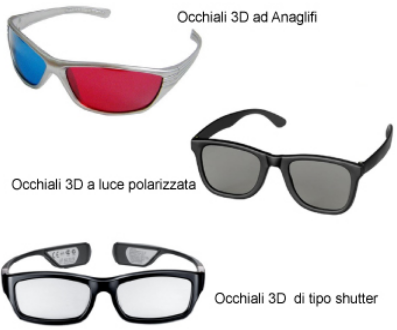
\includegraphics[width=1\columnwidth]{glasses.png}
    \end{minipage}
\end{center}

\section{Powerwall}
Un powerwall è uno schermo grande, ad ultra-alta risoluzione, che è costruito come una matrice di altri display, che
possono essere monitor oppure proiettori. È importante differenziare fra i Powerwalls ed i display che sono
semplicemente grandi.

\paragraph{Prezzo} $\sim$ 20.000 CHF / $5\ m^2$
\section{CAVE}
Cave Automatic Virtual Environment. Ambiente per la realtà virtuale immersiva.
Costituito da una stanza a forma di cubo e proiettori video diretti
tra tre e sei facce.
A differenza degli utenti dei sistemi VR tipo video-arcade, la persona che occupa il CAVE non indossa un HMD 
(Head Mounted Display), ma solamente un paio di cuffie audio. 
Egli si limita a camminare all’interno del CAVE e a interagire con gli oggetti virtuali che incontra mediante dei 
controller tenuti nelle mani. 


Consente agli utenti di:
\begin{itemize}
    \item Analizzare i dati spazialmente correlati
    \item Concentrati sui dati con una soluzione di visualizzazione, software, calcolo e supporto completamente integrata
    \item Senti il modello 3D fluttuare nello spazio, mentre vedi le loro mani e altre persone
    \item Navigare in ambienti a grandezza naturale 
\end{itemize}
Gli utenti di Camera immersiva indossano una coppia di occhiali VR che visualizzano un'immagine 3D tramite stereoscopia . L'effetto 3D viene visualizzato visualizzando due immagini, una per occhio, che consente al cervello di interpretare la profondità degli oggetti. Con l'aiuto di un sistema di tracciamento che registra le azioni della persona all'interno di una sala immersiva, il punto di vista dell'utente è definito per visualizzare le immagini con la giusta prospettiva. 
\paragraph{Prezzo} $\sim$ 30.000 CHF

\subsection{Walking in the Virtual Environment}
In una cave uso una sorta di tapis roulant. 
\paragraph{Prezzo} $\sim$ 400 franchi

\section{Motion Capture (MoCap)}
\subsection{Leap Motion e Kinect}

\subsubsection{Leap Motion Controller}
Piccola periferica USB, pensata per essere piazzata a faccia in su. Può anche essere montata su un headset VR.
Utilizza due microcamere a infrarossi ed ha tre LED infrarossi. Media di accuratezza: 0.7 mm.
Permette di effettuare il tracking delle mani ed è sfruttato per la realtà virtuale.

A differenza del Wiimote di Nintendo e del PlayStation Move di Sony, il Kinect consente al giocatore di controllare
il videogioco senza la necessità di indossare o impugnare alcunché.

\paragraph{Prezzo} $\sim$ 80 dollari


\subsubsection{Kinect}
Sensore di movimento, permette all'utente di interagire con la console / computer mediante una Natural User Interface,
utilizzando dei gesti e dei comandi vocali.
Il sensore è dotato di due videocamere a 480p.
Microsoft ha cessato la produzione di Kinect nel 2017.

\paragraph{Prezzo} $\sim$ 150 dollari

\subsection{MYO}
Sfruttare l'attività muscolare per fornire l'input del computer presenta molti vantaggi rispetto ai dispositivi simili a Kinect che utilizzano telecamere o sensori inerziali. Un nuovo dispositivo di input wireless basato sui gesti che funziona rilevando la firma elettrica delle contrazioni degli avambracci è ora disponibile per il pre-ordine da una nuova società a \textbf{\$150}. La fascia da braccio, soprannominata MYO, viene fornita con un'API per sviluppatori che consente di utilizzare completamente questa sofisticata apparecchiatura.
\subsection{Marcatori passivi}
Sistemi ottici passivi che usano marcatori ricoperti da materiale retroreflettivo che riflette la luce generata da camere posizionate nell'ambiente.
Aggiustando il threshold della camera è possibile riconoscere solo parti abbaglianti ignorando il resto della scena.
Più camere vedono lo stesso marcatore e più è possibile definire in maniera precisa la sua posizione nello spazio 3D (due camere minimo).
Tale sistema implica tipicamente l'uso dalle 2 fino alle 48 camere per cui è parecchio costoso.
\subsection{Radio Frequency (RF)}
\paragraph{Descrizione}
I sistemi RF sono sistemi che rilevano la posizione dell'utilizzatore grazie a delle 
frequenze radio emesse, come i vecchi radar. Con la miglioria di questi devices la 
precisione del rilevamento arriva una precisione di $\sim$10mm.
\paragraph{Vantaggi}
\begin{itemize}
    \item Precisione alta sulla posizione anche a distanza elevata.
    \item Precisione mantenuta su oggetti/soggetti di grossa taglia.
\end{itemize}
\paragraph{Svantaggi}
\begin{itemize}
    \item Facilmente occludibili con un ostacolo tra il rilevatore e l'entità da
    rilevare.
    \item Sconsigliati per motion capture ottimale perchè la precisione è troppo scarsa.
\end{itemize}
\paragraph{Costo} $\sim$300.- CHF (135 Emittore, 175 Ricettore) 

\subsection{Ascension Flock of Birds}
Tecnologia magnetica DC(Direct Current) pulsata per un monitoraggio dei movimenti corporei. È immune da metalli conduttivi non magnetici, è
possibile utilizzare questo tracker intorno all'acciaio inossidabile, al titanio e all'alluminio senza errori di misurazione.
\paragraph{Vantaggi}
\begin{itemize}
    \item Libertà dagli errori di blocco e occlusione.
    \item Non è necessario mantenere una linea visiva libera tra i sensori e il trasmettitore.
    \item Tracciamento simultaneo di tutti i sensori senza degrado nelle velocità di misurazione.
    \item Traccia la testa e le mani contemporaneamente senza ritardi.
    \item La copertura a lungo raggio è disponibile acquistando il trasmettitore a portata estesa (ERT / ERC).
\end{itemize}
\paragraph{Costo}
Prezzo: 1500 franchi circa
\section{Head mounted display - Augmented Reality}
\subsection{Microsoft Hololens}
Il visore si connette al proprio dispositivo mobile o ad un computer con sistema operativo Windows 10 per poter sincronizzare e avviare il dispositivo HoloLens.
Dispone di sensori di movimento, tra cui un giroscopio, un magnetometro e un accelerometro.
È acquistabile in Canada e negli Stati Uniti nella modalità di Development Edition al costo di 3000 dollari, la suite edition 5000 dollari.
L’utente può interagire principalmente con la gesture “air tap” per aprire le app, selezionare gli oggetti e spostare gli ologrammi. Grazie ai sensori che tracciano i movimenti della testa è possibile spostare il cursore con lo sguardo. Il dispositivo supporta anche i comandi vocali, quindi alcune operazioni possono essere completate con l’aiuto di Cortana.
\subsection{Google glasses}
Google Glass è una marca di smart glass, un head mounted display (HMD) che ha la forma di un paio di occhiali. I Google Glass sono stati sviluppati da X (in precedenza Google X)[1] e sono un paio di occhiali dotati di realtà aumentata, tramite i quali è possibile visualizzare informazioni come sugli smartphone senza l'uso delle mani (hands-free). I Glass si operano tramite l'uso di comandi vocali.
Il costo si aggira intorno ai 1000 dollari.

\section{Head mounted display - VR}
Un head-mounted display o HMD, è uno schermo montato sulla testa dello spettatore attraverso un casco ad hoc e può essere monoculare o binoculare.
\subsection{Samsung Gear VR}
Samsung Gear VR è un supporto per display montato come google cardboard.
Ha insieme dei controller per interfacciarsi con il mondo virtuale.
Le sue prestazioni si basano sulle specifiche del telefono inserito al suo interno come schermo.
\paragraph{Vantaggi:}
\begin{itemize}
    \item wireless
    \item basso costo
\end{itemize}
\paragraph{Svantaggi:}
\begin{itemize}
    \item prestazioni, in quanto si appoggia a un telefono e non a un pc.
\end{itemize}
\subsection{Htc Vive}
Questo dispositivo non solo permette di vedere il mondo virtuale mediante un visore ottico, ma grazie ad una nuova tecnologia chiamata "room scale"(tramite cubetti neri che detettano i movimenti del giocatore) trasforma l'ambiente che circonda l'utente in uno spazio 3D in cui può muoversi quasi liberamente. Questa nuova tecnologia associata ad un tracking della testa preciso e a dei comandi di gioco che simulano il movimento delle mani, trasforma la realtà virtuale di HTC Vive in un'esperienza particolarmente immersiva, permettendo all'utente di interagire in maniera quasi completa col mondo di gioco.
La versione PRO è dotato di display a risoluzione più elevata, ora con risoluzione 1440x1600 per-eye, insieme a una seconda fotocamera rivolta verso l'esterno, cuffie collegabili, un microfono per l'analisi dell'annullamento del rumore e un design rinnovato con una forma più "bilanciata", un peso più leggero e un quadrante di dimensionamento. Vive Pro utilizza connettori USB-C anziché USB-A. Comprende anche telecomandi che rintracciano il movimento delle mani, questi telecomandi hanno dei bottoni che servono per interfacciarsi con il mondo virtuale.
\textbf{Prezzo: 499 \$ Prezzo PRO: 1098 \$}
\textbf{Vantaggi} : Buone presentazioni
\textbf{Svantaggi} : Non è wireless e quindi i cavi sono ingombranti e necessità un computer attaccato.
\subsection{Google Cardboard}
Google Cardboard è una visore per la realtà virtuale (VR) sviluppato da Google. E' un head-mounted display per smartphone.  Gli utenti possono creare il proprio visore da componenti semplici e a basso costo utilizzando le specifiche pubblicate da Google oppure acquistarne uno prefabbricato. 
\textbf{Prezzo:} FREE o 8 CHF.
\subsection{Oculus rift}
L'Oculus Rift è il visore di realtà virtuale sviluppato da Oculus VR. Oculus Rift deve essere collegato a un computer per funzionare, un PC che deve avere una determinata potenza per gestire i giochi in realtà virtuale e i mondi virtuali proposti dagli sviluppatori. 
Può comprato con dei telecomandi chiamati Oculus Touch per detettare il movimento delle mani e per dare all’utente un modo per comunicare le proprie azioni/scelte agli utenti.
\paragraph{Vantaggi:}Grafica vivida e fluida.
\paragraph{Svantaggi:}
\begin{itemize}
    \item Necessità di essere attaccato a un pc
    \item Cavi ingombranti
\end{itemize}
\paragraph{Prezzo: 399 \$}
\section{Haptics}
Dispositivo VR che da un feedback tattile che può anche essere una forza opposta che non ti fa chiudere la mano quando nel mondo virtuale prendi un oggetto.
Un esempio di haptics che pero non ha la forza resistente è VR Glove chiamati Plexus che ha un feedback tattile. Prezzo 250\$.
\subsection{Reactive Grip Motion Controller}
Sono dei controller che hanno nel manico dei piatti magnetici che simulano le forze di frizione che si avrebbero quando terresti l'oggetto che nel mondo virtuale stai tenendo.
\begin{center}
    \begin{minipage}{\columnwidth}
        \centering
        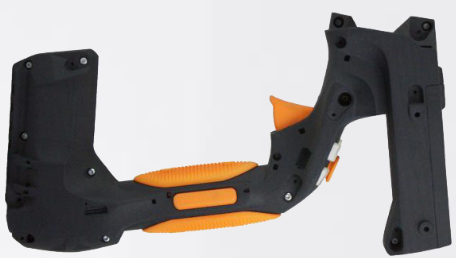
\includegraphics[width=3cm]{reactiveGrip.png}
    \end{minipage}
\end{center}
\paragraph{Prezzo: 78\$}
\subsection{Haptic Mask(bHaptics)}
E' una fascetta che si mette in testa per sentire fisicamente un tocco in testa quando si riceve un colpo nel medesimo.
\subsection{Haptic Sleeve(bHaptics)}
Uguale a Haptic Mask, ma sento il feedback sul braccio.
\subsection{Haptic Vest(bHaptics)}
Uguale a Haptic Mask, ma sul busto.
\paragraph{Il prezzo dell'intera suit è 549 \$} 
\section{Altre tecnologie}
\subsection{Artoolkit}
ARToolKit is an open-source computer tracking library for creation of strong augmented reality applications that overlay virtual imagery on the real world.
Prezzo: 100\$
\subsection{Skybox}
\paragraph{Descrizione} 
Una Skybox è una tipologia speciale di texture che viene applicata all'iterno di un 
cubo, nel quale sarà contenuta la scena. Si utilizza per dare una texture ad elementi
esterni o irraggiungibili dall'utente. 
\paragraph{Vantaggi}
\begin{itemize}
    \item Facile da implementare.
    \item Facile codificare le coordinate delle texture anche a mano.
    \item Facile e veloce da disegnare.
\end{itemize}
\paragraph{Svantaggi}
\begin{itemize}
    \item Si possono avere problemi con la prospettiva e soprattuto con gli angoli.
    \item Può essere difficile disegnare una Skybox del quale non si noti il cubo.
\end{itemize}
\paragraph{Costo} Potenzialmente gratuita.
\subsection{Skydome}
\paragraph{Descrizione} 
Una Skydome è come una Skybox ma invece che essere applicata su un cubo viene applicata
su una semisfera.
\paragraph{Vantaggi}
\begin{itemize}
    \item È relativamente semplice disegnarla.
    \item Flessibile perchè alto numero di vertici.
    \item Meno problemi di prospettiva 
\end{itemize}
\paragraph{Svantaggi}
\begin{itemize}
    \item Numero di vertici alto quindi più lenta.
\end{itemize}
\paragraph{Costo} Potenzialmente gratuita.
\subsection{OpenVR e SteamVR}
OpenVR è un software development kit ed API che permette di comunicare con dell'
hardware per VR da codice e quindi inviare e ricevere dati. SteamVR è invece un 
applicativo che permette la trasmissione di un ambiente VR che può fare da interfaccia
tra OpenVR ed il visore effettivo.
\subsubsection{TrinusVR Cardboard}
TrinusVR fa da comunicatore tra il pc ed il telefono, si può scegliere SteamVR come 
sorgente dei dati ed una volta connessi si avrà la trasmissione sul telefono.
\paragraph{Server}
Lato pc si usa TrinusVR Cardboard Server come software che farà sorgente e Server.
\paragraph{Client} 
Lato telefono usiamo TrinusCBVR come applicazione che riceverà i dati e trasmetterà
le immagini (differenti per ogni occhio e quindi lo stereoscopic rendering).
% // QUESTO E' QUELLO CHE VA INSERITO:

% DI QUESTI SOTTO POSSIAMO INSERIRE: il "giro che abbiamo fatto nel nostro progetto"

% DI QUESTI SOTTO POSSIAMO INSERIRE: qualche utilizzo reale
% Object picking

% VERIFICARE E AGGIUNGERE IL MINIMO FPS:
% VR deve garantire almeno 60 frame per occhio (120 frame/secondo)

% DA AGGIUNGERE SE NON C'E' GIA' NEL LEAP MOTION:
% il leap motion può essere montato anche sopra gli headset in modo che vedi le mani nell’ambiente virtuale. Usa gli infrassossi, verificare numero camere

% CERCARE QUALCOSA SU INTERNET:
% Tuta di pura, la giacchetta (quando ti sparano)

%AGGIUNGERE:
% sensori film
% parco giochi jonny
% uforia
% aggiungere nei motion capture le tecnologie per il cinema eccetera (brief history slide 20-21)
% Dalla slide 28 alla 33 della brief history ci sono tutte le applicazioni della realtà virtuale che possiamo inserire

\end{multicols}
\end{document}
